\documentclass[letter,10pt]{article}
\usepackage{balance}
\usepackage[utf8]{inputenc} 
\usepackage[T1]{fontenc}
\usepackage[spanish]{babel}
\usepackage{enumerate}
\usepackage{pdfpages}
\usepackage{graphicx}
\usepackage{multicol}
\usepackage{multirow}
\usepackage{float}
\usepackage{fancyhdr}
\usepackage{latexsym}
\usepackage{amsmath}
\usepackage{amssymb} 
\usepackage[top=2cm,bottom=5cm,left=2cm,right=1.5cm]{geometry}


\title{\bf IPM407: Modelación Computacional con Algoritmos Rápidos\\{\bf Métodos Basados en Transformada de Fourier}\\{\it Departamento de Ingeniería Mecánica,}\\{\it Universidad Técnica Federico Santa María\\Valparaíso, Chile}}

\author{Profesor: Christopher Cooper \\ Alumno: Javier Gómez G.}
\date{15/06/2017}

\pagestyle{empty}

\pagestyle{fancy}
\headheight = 80pt 
\fancyhead[R] 
{
\begin{minipage}{2cm}

\includegraphics[scale=0.35]{img/usm.jpg}
\end{minipage}
\hspace{0.05\linewidth}
\begin{minipage}{1.8cm}

\includegraphics[scale=0.5]{img/mecanica.jpg}
\end{minipage}
}
\fancyhead[L] 
{ Universidad Técnica Federico Santa Maria\\ Departamento Ingeniería Civil Mecánica\\ Casa Central}

\fancyfoot[R] 
{ Autor: Javier Gómez}

\begin{document}
\maketitle
\begin{minipage}{0.5\linewidth}
\begin{figure}[H]
\centering

\includegraphics[scale=0.5]{img/usm1.jpg}
\end{figure}
\end{minipage}
      \hspace{0.01\linewidth}
      \begin{minipage}{0.3\linewidth}
\begin{figure}[H]
\centering

\includegraphics[scale=0.8]{img/mecanica.jpg}
\end{figure}
\end{minipage}

\thispagestyle{empty}

\newpage

{\bf\Large Resumen:}\\

\indent Este Informe contiene información sobre los resultados obtenidos al realizar el estudio de la implementación de métodos Multi mallas para acelerar el calculo en códigos para métodos de relajación. Para dicha tarea, este informe parte por dar una pequeña descripción del equipo y el que se utilizaron. Posteriormente se describe la situación de estudio a partir de un caso particular de la ecuación de Poisson el cual se discretiza en base a un esquema de diferencias finitas centrado de orden cuadrático. Luego de la descripción del caso estudiado se exponen los codigos utilizados para llevar a cabo esa labor.\\
\indent Posterior a todas las descripciones preliminares se exponen los resultados obtenidos a partir del código desarrollado, estos exponen partiendo de los resultados cualitativos para un campo escalar teórico y para las aproximaciones usando los métodos de relajación y las formas aceleradas de dichos métodos, luego se exponen cuadros resumen de los resultados cuantitativos para posteriormente pasar a gráficos que reflejan la complejidad algoritmica de los métodos.\\
\indent En base a los resultados expuestos en este trabajo se da lugar a la discusión de los análisis y conclusiones a las que se llegaron luego de desarrollar los pasos descritos previamente.\\ 
\\

{\bf\Large Objetivos:}\\
\begin{itemize}
\item {\bf Principal:} Implementar Métodos multi-mallas para resolver sistemas lineales reconociendo sus ventajas y desventajas.\\
\item {\bf Específicos:}
\begin{itemize}
\item Reconocer las cualidades de los métodos de relajación.
\item Implementar {\it V-cycle} y establecer su ventaja respecto a los métodos de relajación simple.
\item Implementar {\it Full-multigrid-scheme} y reconocer sus ventajas y desventajas respecto a {\it V-cycle} y relajación simple.
\item Comprobar que se cumplen las predicciones teóricas con respecto a los tiempos de cálculos.
\end{itemize}
\end{itemize}

\newpage

\tableofcontents

\newpage

\section{Computador y lenguaje utilizado}

El pc utilizado para realizar los cálculos fue:

\begin{figure}[H]
\centering
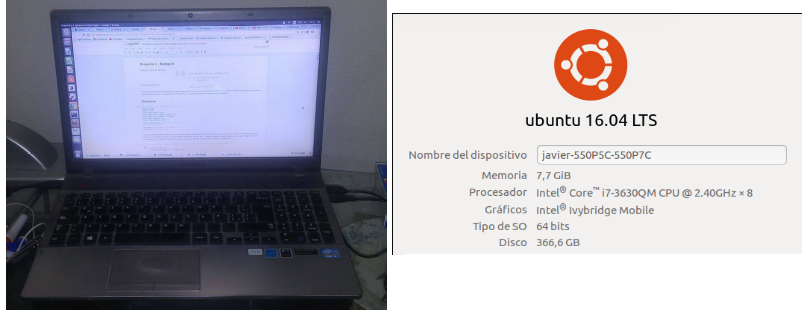
\includegraphics[scale=0.8]{img/mipc2.png}
\caption{Presentación y resumen de las características del PC a utilizado para hacer los cálculos}
\label{mipc}
\end{figure}

En cuanto al lenguaje utilizado para realizar los códigos fue python. Los codigos se escribieron en notbooks interactivos conocidos como {\bf ipython notebook} mediante la interfaz de jupyter.

\begin{figure}[H]
\centering

\includegraphics[scale=0.8]{img/lemguaje.jpg}
\caption{Python versión 2.7 y Jupyter versión 4.2.0}
\label{legunaje}
\end{figure}

\section{Desarrollo}

\subsection{Discretización y Esquemas}

Con el fin de llevar a cabo los objetivos, se estudio el comportamiento de la siguiente ecuación de Poisson:

\begin{equation}
\frac{\partial^2 u}{\partial x^2}+\frac{\partial^2 u}{\partial y^2} = -2[(1-6x^2)y^2(1-y^2)+(1-6y^2)x^2(1-x^2)]
\label{poisson}
\end{equation}
$$u=0\quad en\quad x=0,x=1,y=0,y=1$$
$$0\leq x \leq 1 \quad 0\leq y \leq 1$$

Que tiene solución analítica:

\begin{equation}
u(x,y) = (x^2-x^4)(y^4-y^2)
\label{solucionanalitica}
\end{equation}

Para resolver de forma numérica la EDP de la ecuación (\ref{poisson}), se utilizó un esquema de discretización por diferencias finitas centrada de orden dos para las segundas derivadas, es decir:

\begin{equation}
\frac{\partial^2 u}{\partial x^2}=\frac{u_{i-1,j}-2u_{i,j}+u_{i+1,j}}{\Delta x^2} + o(\Delta x^2) \quad y \quad \frac{\partial^2 u}{\partial y^2}=\frac{u_{i,j-1}-2u_{i,j}+u_{i,j+1}}{\Delta y^2}+ o(\Delta y^2)
\label{discret}
\end{equation}

\noindent donde en este caso $o(\Delta x^2)$ y $o(\Delta y^2)$ son el orden del error de la discretización producto de la expansión en serie de Taylor para las segundas derivadas de $u$.\\

Ademas, de ahora en adelante y con el fin de simplificar la notación, se dirá que:

\begin{equation}
f_{i,j}=f(x_{i},y_j) = -2[(1-6x_i^2)y_j^2(1-y_j^2)+(1-6y_j^2)x_i^2(1-x_i^2)]
\label{fdef}
\end{equation} 

En este trabajo se pretende resolver el sistema $Au=f$ obtenido al reemplazar las discretizaciones de (\ref{discret}) en (\ref{poisson}) y usando métodos de relajación como Jacobi, Gauss-Seidel y Red-Black Gauss-Seidel \cite{iter}. Luego, considerando que $v$ es una aproximación de $u$ y representado los métodos de iteración libre de matrices, se tiene:

\begin{equation}
Jacobi: \quad v_{i,j}^{k+1} = \frac{1}{2}\frac{\Delta x^2 \Delta y^2}{\Delta y^2 + \Delta x^2}\left[-f_{i.j}+\left(\frac{u_{i-1,j}^k+u_{i+1,j}^k}{\Delta x^2}+\frac{u_{i,j-1}^k+u_{i,j+1}^k}{\Delta y^2} \right)\right]
\end{equation}

\begin{equation}
Gauss-Seidel: \quad v_{i,j}^{k+1} = \frac{1}{2}\frac{\Delta x^2 \Delta y^2}{\Delta y^2 + \Delta x^2}\left[-f_{i.j}+\left(\frac{u_{i-1,j}^{k+1}+u_{i+1,j}^k}{\Delta x^2}+\frac{u_{i,j-1}^{k+1}+u_{i,j+1}^k}{\Delta y^2} \right)\right]
\end{equation}

Para Red-Black Gauss-Seidel se dividen la malla en nodos $rojos$ y $negros$ (Figura \ref{RBGSDIBUJO}), se resuelven los nodos $rojos$ con $Jacobi$ y luego, usando los resultados calculados con $Jacobi$ se calculan los nodos $negros$ usando $Gauss-Seidel$.

\begin{figure}[H]
\centering
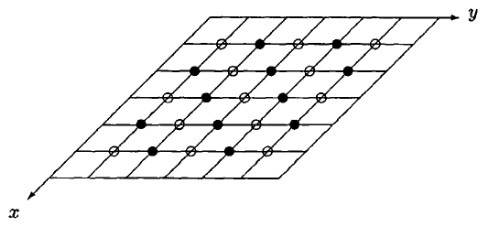
\includegraphics[scale=0.8]{img/RBGSDIBUJO}
\caption{Esquema de una malla dividida en nodos para aplicar RB-GS. Los nodos "rojos" en este esquema son los blancos.}
\label{RBGSDIBUJO}
\end{figure}

\subsection{Códigos}

Antes de escribir los algoritmos se importan las librerías de $numpy$, $matplotlib$, $time$ y $numba$, para definir arreglos y algunas operaciones matemáticas, hacer gráficos, medir tiempo y acelerar la compilación de algunas rutinas, respectivamente.

\begin{figure}[H]
\centering
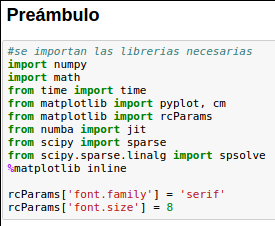
\includegraphics[scale=0.8]{img/preambulo}
\caption{Códigos para importar librerías a utilizar}
\end{figure}

Antes de definir los algoritmos para los métodos de relajación es necesario definir algunas funciones que se ocuparan a lo largo de todo el código, estas funciones se pueden ver en la Figura \ref{funcionesprel}. Que hace cada una de las funciones de la Figura \ref{funcionesprel} son descritas en los comentarios que aparecen en la figura

\begin{figure}[H]
\centering
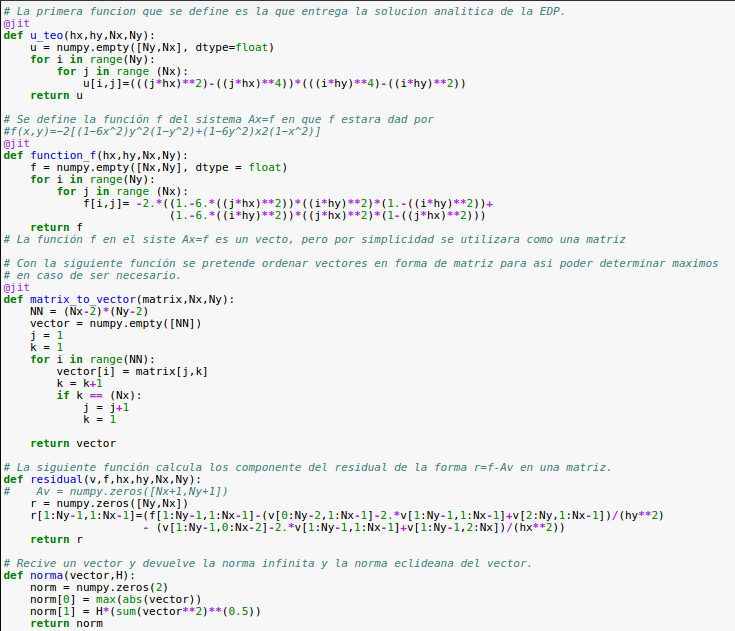
\includegraphics[scale=0.9]{img/funciones}
\caption{Funciones preliminares}
\label{funcionesprel}
\end{figure} 

A continuación se presentan la funciones que realizan las relajaciones:

\begin{figure}[H]
\centering
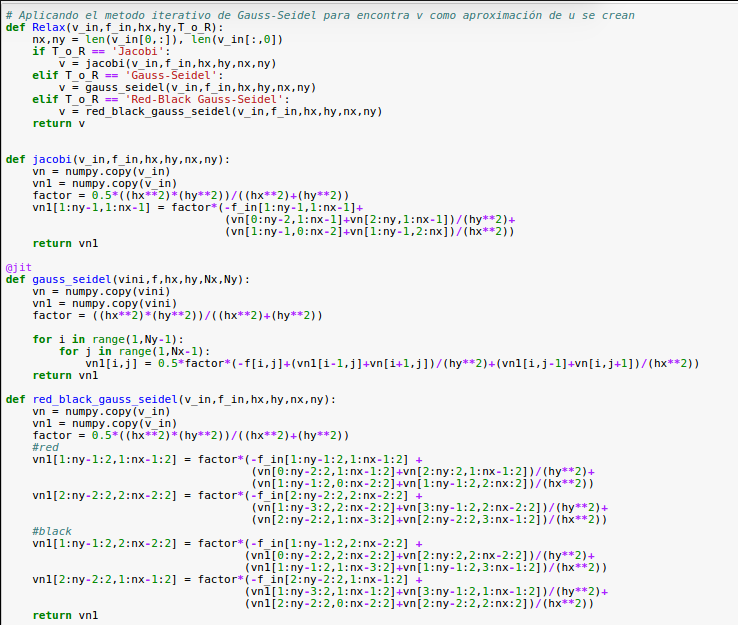
\includegraphics[scale=0.85]{img/relajaciones}
\caption{Códigos para las relajaciones}
\label{relax}
\end{figure}

Posteriormente se escriben los códigos para V-cycle y para Multigrid, pero antes -debido al movimiento entre mallas finas y gruesas- es necesario escribir códigos para transferencia de mallas. 

\begin{figure}[H]
\centering 
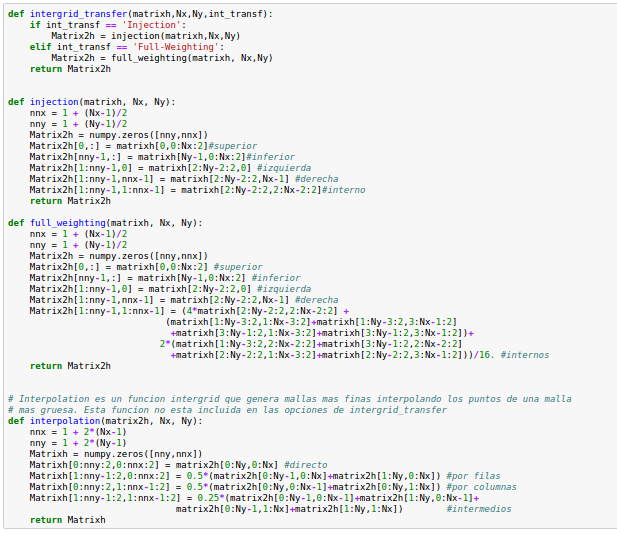
\includegraphics[scale=1.1]{img/intergridcode}
\caption{Los codigos de transferencia de malla son $injection$ y $full weighting$ para ir de mallas finas a gruesas e $interpolation$ para ir de mallas gruesas a finas}
\label{intergridcode}
\end{figure}

\begin{figure}[H]
\centering
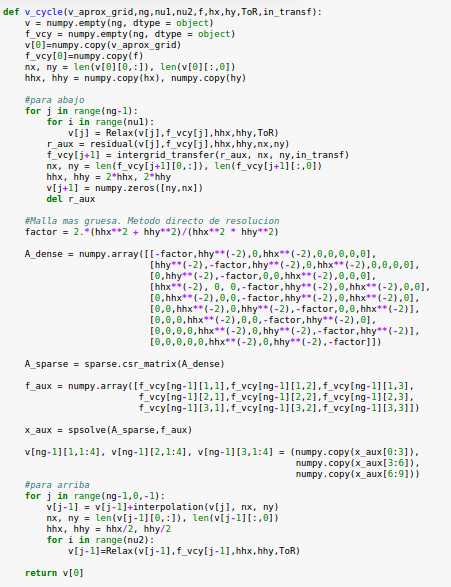
\includegraphics[scale=1.3]{img/vcyclecode}
\caption{Codigos para ciclo V. La malla mas gruesa se resuelve con métodos directos.}
\label{ciclovcode}
\end{figure}

\begin{figure}[H]
\centering
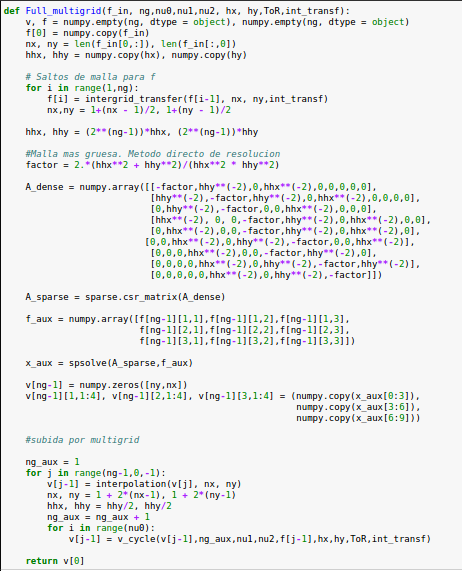
\includegraphics[scale=1.3]{img/multigridcode}
\caption{Codigos para Full-Multigrid. Al igual que en ciclo-V para la malla mas gruesa se resuelve por métodos directos.}
\label{multigridcode}
\end{figure}

Las funciones anteriormente definidas (relajaciones, cambios de malla, ciclo-V y Full-Multigrid) fueron pensadas inicialmente para ocupar mallas con distinta cantidad de nodos por eje ($N_x \neq N_y$) y que el espacio entre nodos también sea distinta ($\Delta x \neq \Delta y$) pero a lo largo de la programación esa generalidad se perdió y solo es posible utilizar estos codigos cuando se cumple que $N_x = N_y$ y $\Delta x = \Delta y$.\\

En $Ciclo-V$ y en $Full-Multigrid$ se fuerza a que la malla mas gruesa sea de $N_x=N_y=5$ en la cual, solo los puntos centrales de la malla son incognitas ya que los bordes son definidos por las condiciones de contorno, en este sentido se genera un sistema de nueve ecuaciones y nueve incognitas.\\

Además, $Ciclo-V$ cuenta con los parámetros $\nu_1$ y $\nu_2$ que son la cantidad de relajaciones cuando va cambiando de matrices finas a gruesas y gruesas a finas respectivamente. Para $Full-Multigrid$ además se define $\nu_0$ que es la cantidad de $ciclos_V$ que se realizan mientras se va "subiendo" desde las mallas gruesas a las finas.

\section{Resultados}

\subsection{Validación}
Para saber si los resultados obtenidos por los códigos es apropiado primero se hace una validación cualitativa.\\

El campo $u$ teorico se ve de la siguiente forma

\begin{figure}[H]
\centering
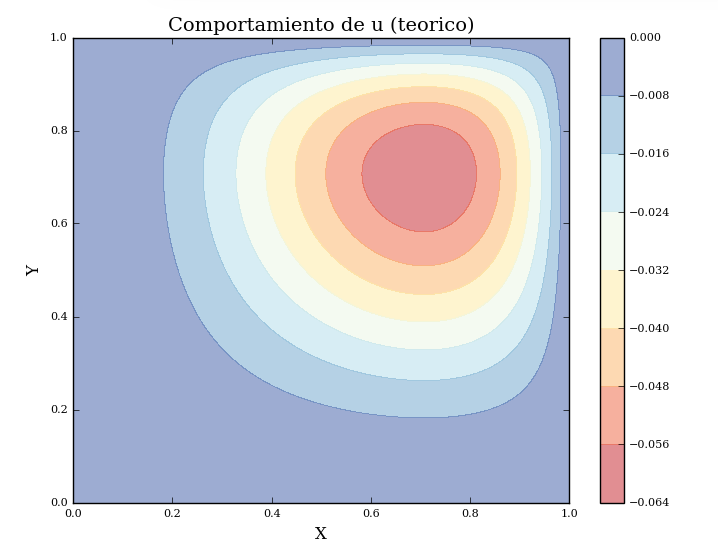
\includegraphics[scale=0.6]{img/u_teorico}
\caption{Campo $u$ teórico}
\label{cualitteorico}
\end{figure}

Las aproximaciones $v$ de $u$ con los distintos métodos y una tolerancia para el residual de $10^{-8}$ se ven de la siguiente forma.

\subsubsection{Relajaciones Simples}

\begin{table}[H]
\centering
\caption{Recopilación cualitativa de $v$ para los metodos de relajación simple}
\begin{tabular}{|l|l|}
\hline
\multicolumn{2}{|c|}{Jacobi} \\ \hline
N=65 & N=129 \\ 
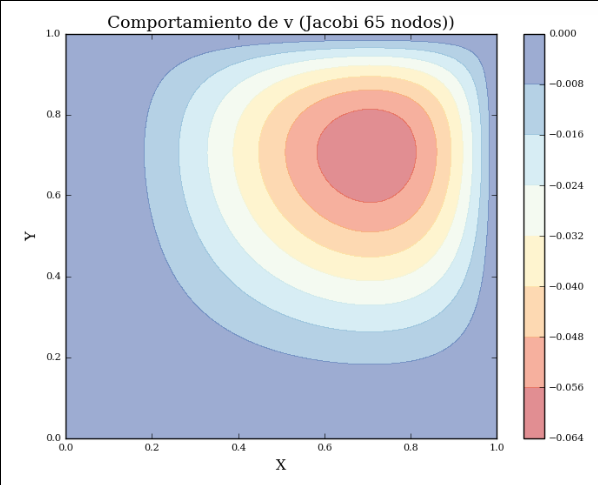
\includegraphics[scale=0.4]{img/v_jacobi65N} & 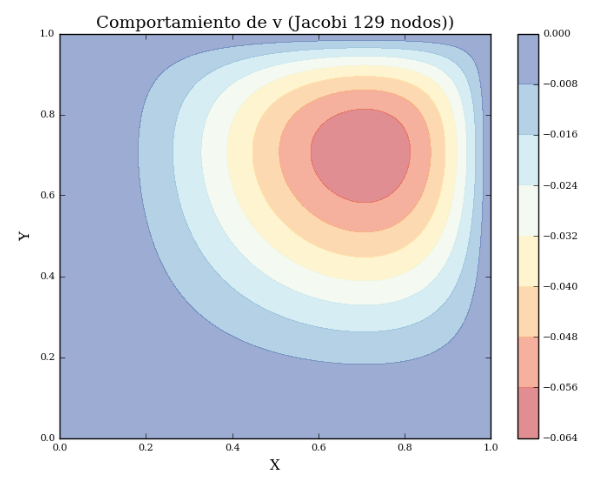
\includegraphics[scale=0.4]{img/v_jacobi129N} \\ \hline
\multicolumn{2}{|c|}{Gauss-Seidel} \\ \hline
N=65 & N=129 \\ 
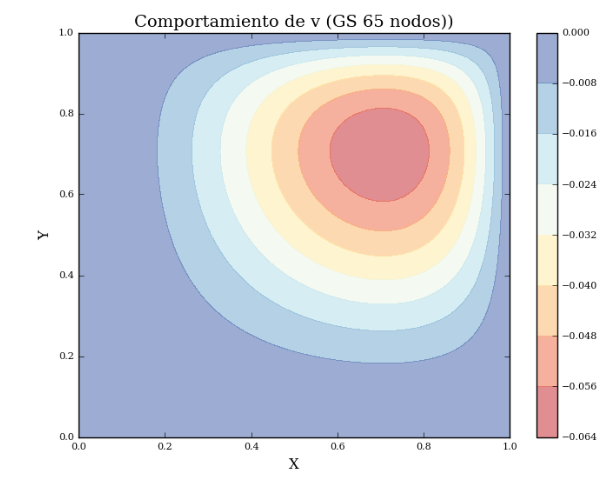
\includegraphics[scale=0.4]{img/v_GS65N} & 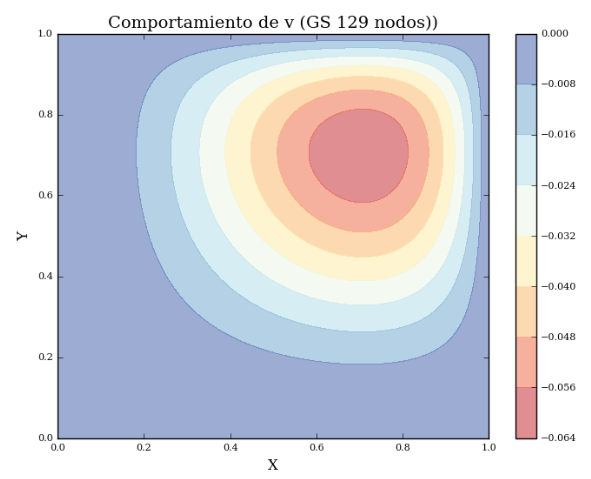
\includegraphics[scale=0.4]{img/v_GS129N} \\ \hline
\multicolumn{2}{|c|}{Red-Black Gauss-Seidel} \\ \hline
N=65 & N=129 \\ 
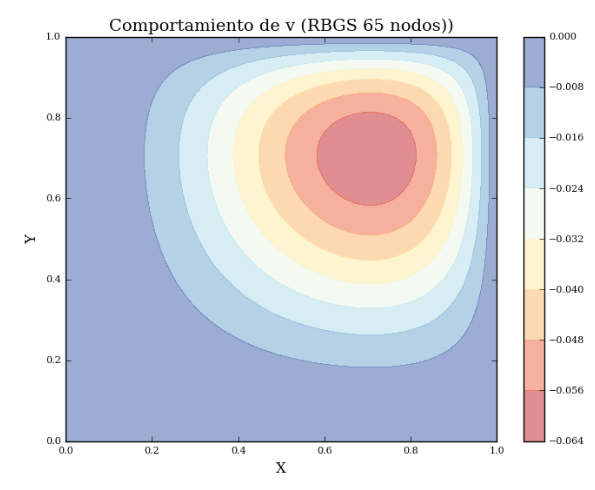
\includegraphics[scale=0.4]{img/v_RBGS65N} & 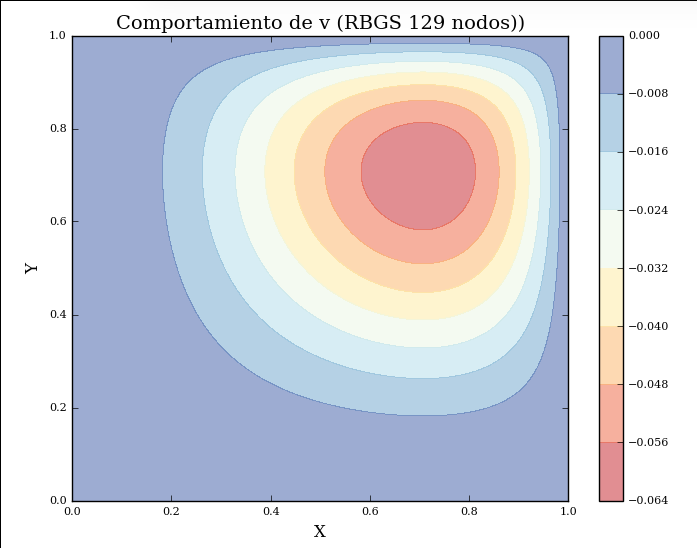
\includegraphics[scale=0.35]{img/v_RBGS129N} \\ \hline
\end{tabular}

\label{cualitrelaxsimple}
\end{table}

\subsubsection{V-Cycle}

\begin{table}[H]
\centering
\caption{Recopilación cualitativa de $v$ para $V-Cycle$ usando i$\nu_1=2$, $\nu_2=2$}
\begin{tabular}[t]{|c|c|c|}
\hline
\multicolumn{3}{|c|}{Inyección} \\ \hline
%\multicolumn{3}{|c|}{N=65} \\ \hline
Jacobi & Gauss-Seidel & R-B Gauss-Seidel \\ \hline
\multicolumn{3}{|c|}{N=65} \\ \hline 
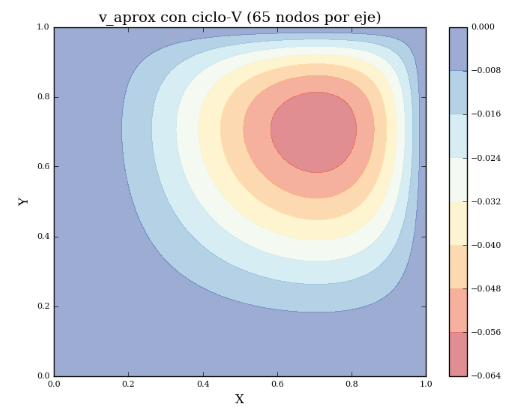
\includegraphics[scale=0.34]{img/v_cvjacobi65Ninjection} &
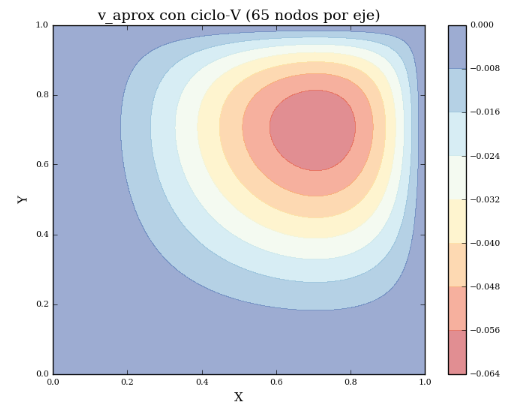
\includegraphics[scale=0.34]{img/v_cvGS65Ninjection} &
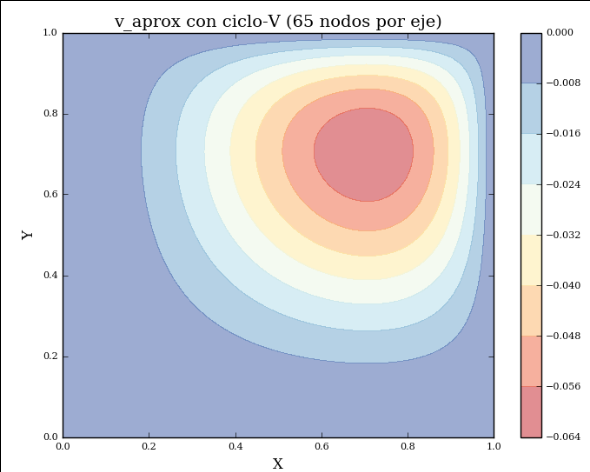
\includegraphics[scale=0.30]{img/v_cvRBGS65Ninjection} \\ \hline
\multicolumn{3}{|c|}{N=129} \\ \hline
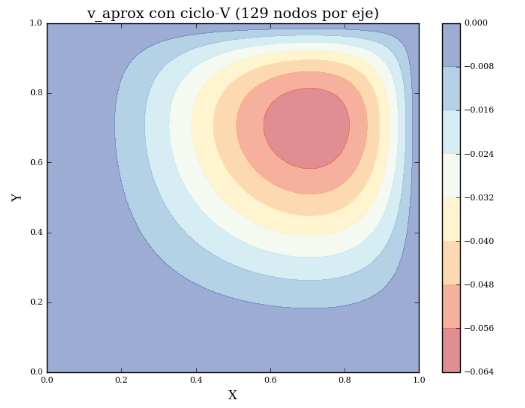
\includegraphics[scale=0.34]{img/v_cvjacobi129Ninjection}&
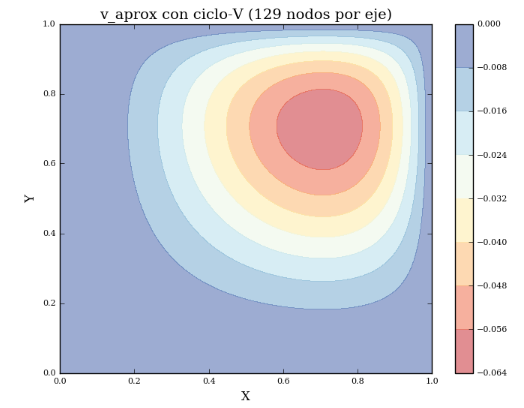
\includegraphics[scale=0.34]{img/v_cvGS129Ninjection}&
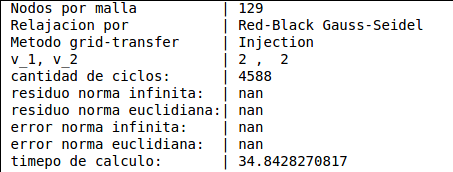
\includegraphics[scale=0.40]{img/v_cvRBGS129Ninjection} \\ \hline
\multicolumn{3}{|c|}{Full-Weighting} \\ \hline
%\multicolumn{3}{|c|}{N=65} \\ \hline
Jacobi & Gauss-Seidel & R-B Gauss-Seidel \\
\multicolumn{3}{|c|}{N=65} \\ \hline 
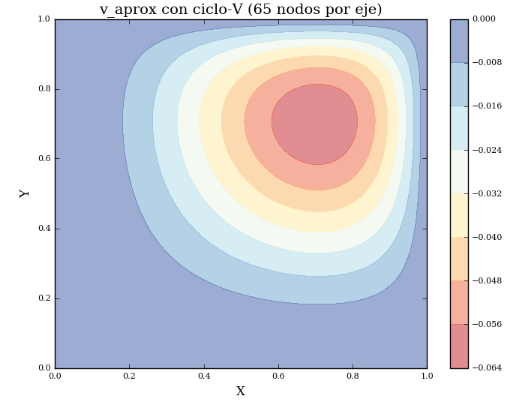
\includegraphics[scale=0.34]{img/v_cvjacobi65NFW} &
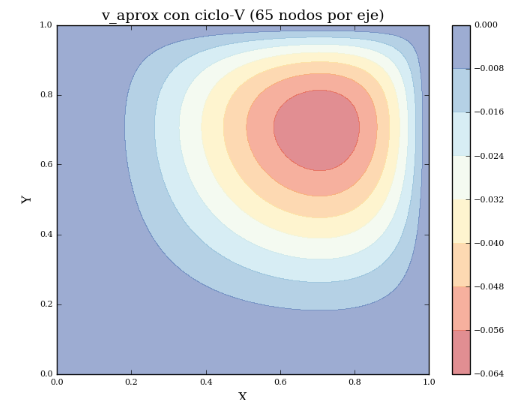
\includegraphics[scale=0.34]{img/v_cvGS65NFW} &
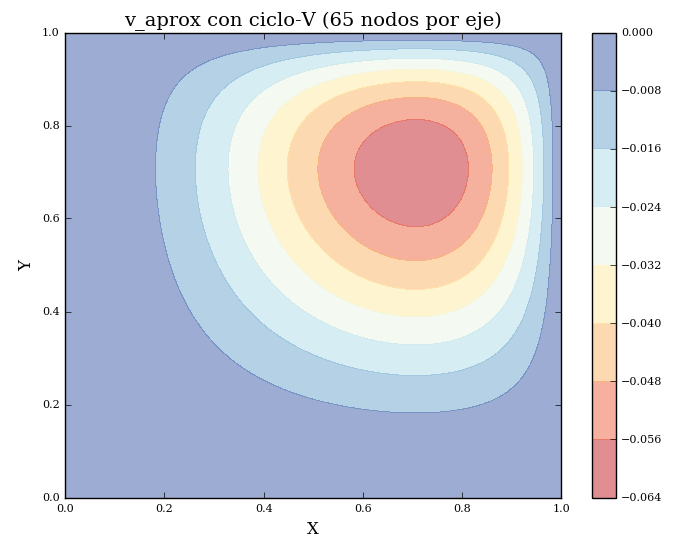
\includegraphics[scale=0.26]{img/v_cvRBGS65NFW} \\ \hline
\multicolumn{3}{|c|}{N=129} \\ \hline
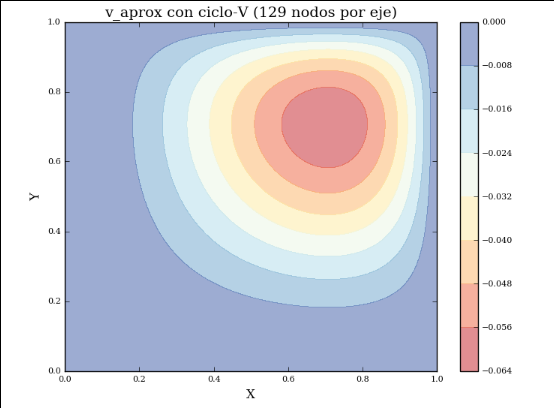
\includegraphics[scale=0.38]{img/v_cvjacobi129NFW}&
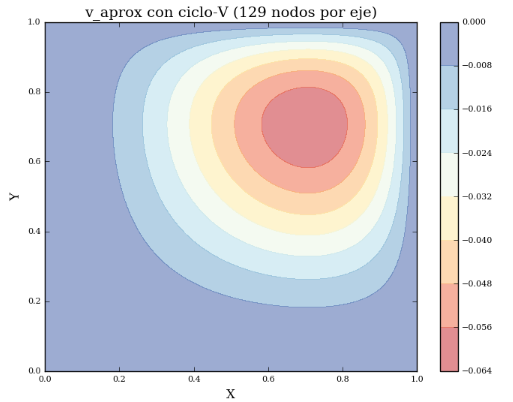
\includegraphics[scale=0.38]{img/v_cvGS129NFW}&
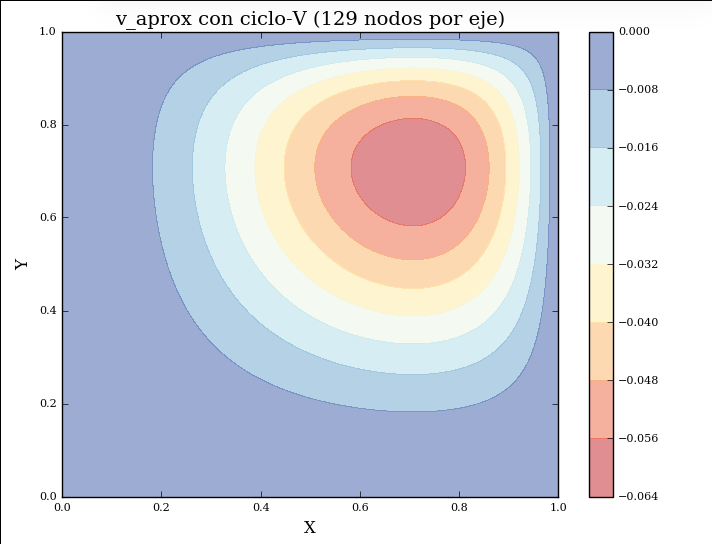
\includegraphics[scale=0.3]{img/v_cvRBGS129NFW} \\ \hline
\end{tabular}

\label{cualitvc}
\end{table}



\subsubsection{Full-Multigrid}
Para Full-Multigrid, debido a que no se consigue el valor cualitativo adecuado para los parametros $\nu$ utilizados, es que solo se muestra como se ve el campo para $129$ nodos por eje

\begin{table}[H]
\centering
\caption{Recopilación cualitativa de $v$ para $Multigrid$ usando $\nu_1=2$, $\nu_2=2$ y $\nu_0=1$}
\begin{tabular}[t]{|c|c|c|}
\hline
\multicolumn{3}{|c|}{Por inyección} \\ \hline
Jacobi & Gauss-Seidel & R-B Gauss-Seidel\\ \hline 
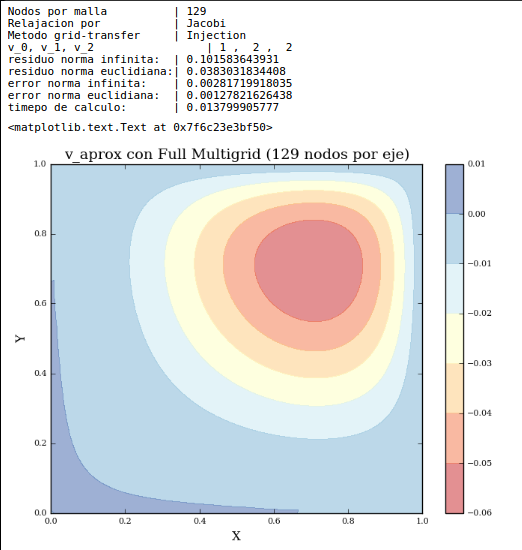
\includegraphics[scale=0.38]{img/fmg/mgjacobi129Ninjection}& 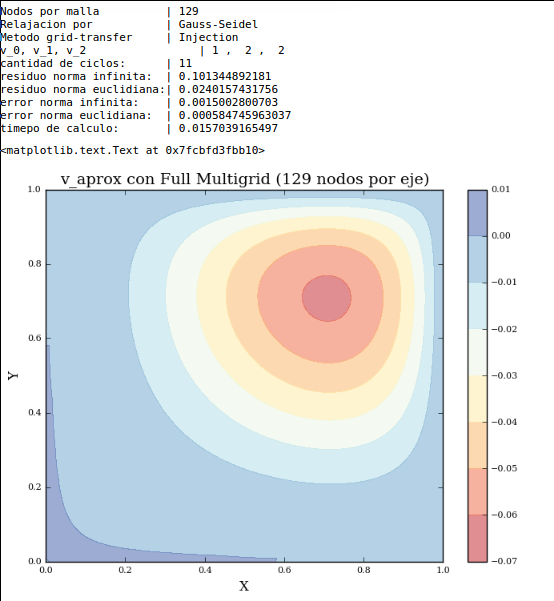
\includegraphics[scale=0.35]{img/fmg/mgGS129Ninjection}&
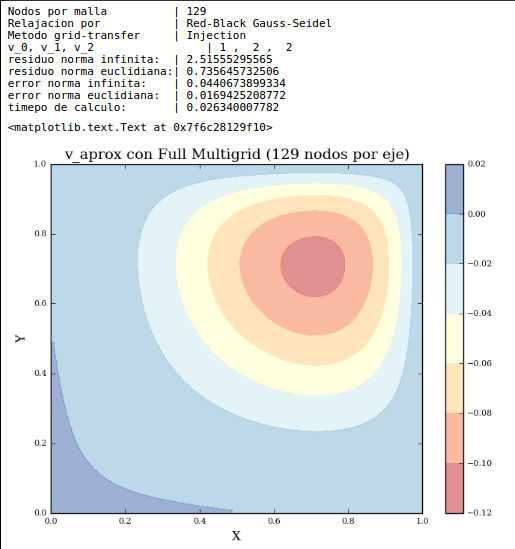
\includegraphics[scale=0.38]{img/fmg/mgRBGS129Ninjection} \\ \hline
\multicolumn{3}{|c|}{Por Full-Weighting} \\ \hline
Jacobi & Gauss-Seidel & R-B Gauss-Seidel\\ \hline 
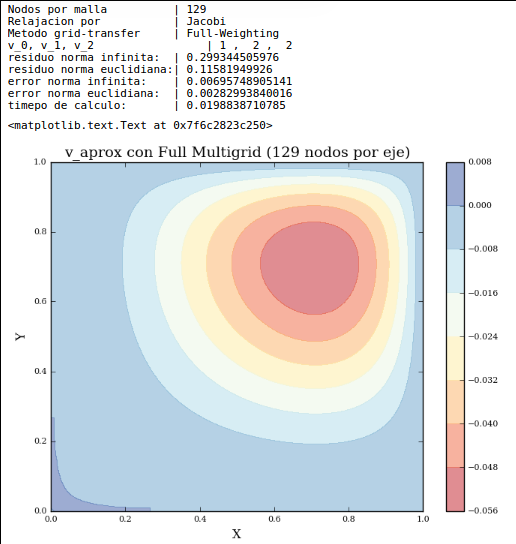
\includegraphics[scale=0.38]{img/fmg/mgjacobi129NFW}& 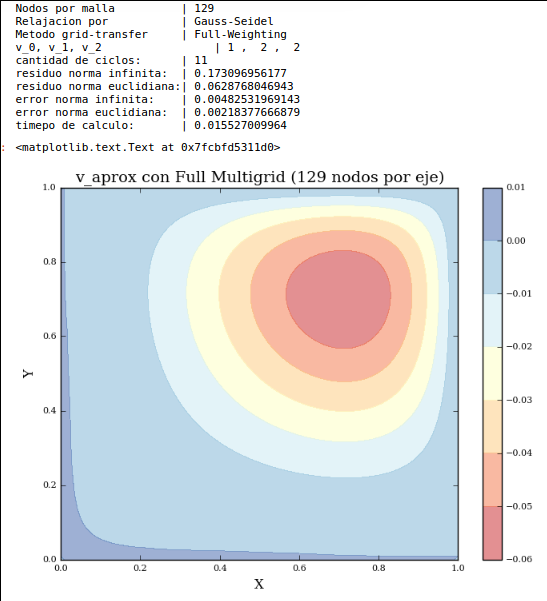
\includegraphics[scale=0.35]{img/fmg/mgGS129NFW}&
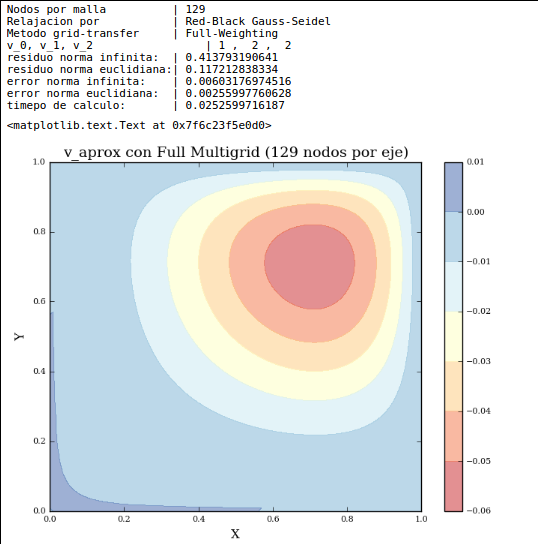
\includegraphics[scale=0.38]{img/fmg/mgRBGS129NFW} \\ \hline

\end{tabular}

\label{cualitmg221}
\end{table}

Si se cambian los valores de $\nu$

\begin{table}[H]
\centering
\caption{Resultados cualitativos para $Multigrid$ usando Gauss-Seidel, $\nu_1=10$, $\nu_2=10$ y $\nu_0=5$}
\begin{tabular}[t]{|c|c|}
\hline
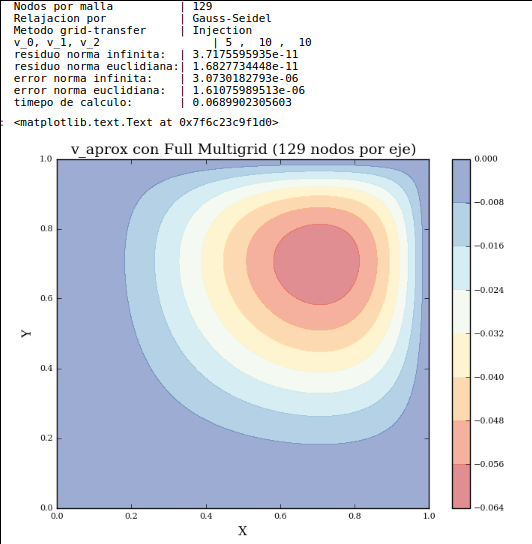
\includegraphics[scale=0.55]{img/fmg/inject10105}& 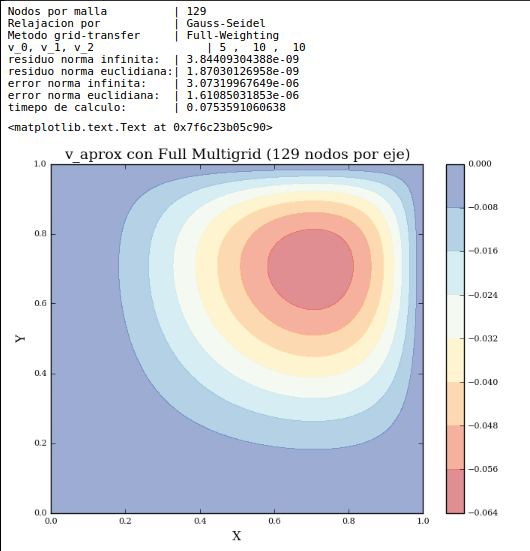
\includegraphics[scale=0.55]{img/fmg/FW10105}\\ \hline
\end{tabular}

\label{cualitmg10105}
\end{table}

\begin{table}[H]
\centering
\caption{Resultados cualitativos para $Multigrid$ usando Gauss-Seidel, $\nu_1=10$, $\nu_2=10$ y $\nu_0=4$}
\begin{tabular}[t]{|c|c|}
\hline
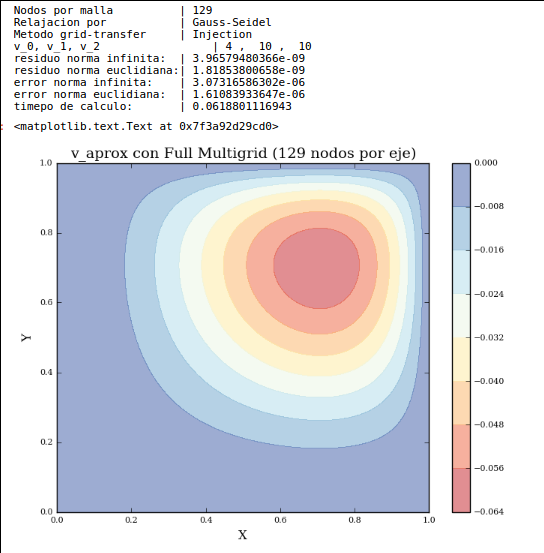
\includegraphics[scale=0.55]{img/fmg/inject10104}& 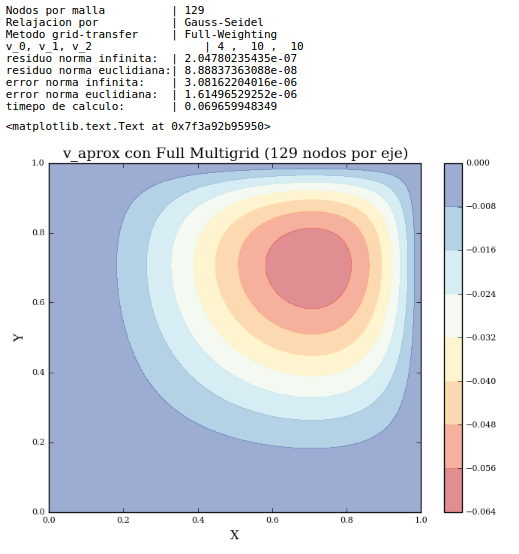
\includegraphics[scale=0.55]{img/fmg/FW10104}\\ \hline
\end{tabular}

\label{cualitmg10104}
\end{table}

\subsection{Tiempo, Residuo y Errores}

\begin{table}[H]
\centering
\caption{Tabla resumen para la aplicación de los métodos de relajación}
\begin{tabular}[t]{|l|r|r|r|r|r|}
\hline
\multicolumn{ 1}{|c|}{Jacobi} & \multicolumn{1}{l|}{Nodos} & \multicolumn{1}{l|}{Tiempo [s]}& \multicolumn{1}{l|}{Ciclos} & \multicolumn{1}{c|}{$||r||_{\infty}$} & \multicolumn{1}{c|}{$||e||_{\infty}$} \\ \cline{ 2- 6}
\multicolumn{ 1}{|l|}{} &9 & 0.035& 230 & 9.65E-09 & 0.0007639 \\ \cline{ 2- 6}
\multicolumn{ 1}{|l|}{} & 17 & 0.155 & 939 &9.81E-09 & 0.0001967 \\ \cline{ 2- 6}
\multicolumn{ 1}{|l|}{} & 33 & 1.117 & 3772 &9.98E-09 & 4.92E-05 \\ \cline{ 2- 6}
\multicolumn{ 1}{|l|}{} & 65 & 13.873 &15107&9.99E-09 & 1.23E-05 \\ \cline{ 2- 6}
\multicolumn{ 1}{|l|}{} & 129 & 203.512 &60445 &1.00E-08 & 3.07E-06 \\ \cline{ 2- 6}
\multicolumn{ 1}{|l|}{} & 257 & 3098.59 & 241797 & 1.00E-08 &7.69E-07 \\ \hline

\multicolumn{ 1}{|c|}{GS} & \multicolumn{1}{l|}{Nodos} & \multicolumn{1}{l|}{Tiempo [s]}& \multicolumn{1}{l|}{Ciclos} & \multicolumn{1}{c|}{$||r||_{\infty}$} & \multicolumn{1}{c|}{$||e||_{\infty}$} \\ \cline{ 2- 6}
\multicolumn{ 1}{|l|}{} &9 & 0.016& 118 & 9.22E-09 & 0.0007639 \\ \cline{ 2- 6}
\multicolumn{ 1}{|l|}{} & 17 & 0.097 & 474 &9.83E-09 & 0.0001967 \\ \cline{ 2- 6}
\multicolumn{ 1}{|l|}{} & 33 & 0.511 & 1894 &1.00E-09 & 4.92E-05 \\ \cline{ 2- 6}
\multicolumn{ 1}{|l|}{} & 65 & 6.675&7569 & 9.99E-09 & 1.23E-05 \\ \cline{ 2- 6}
\multicolumn{ 1}{|l|}{} & 129 & 100.535& 30252 & 1.00E-08 & 3.07E-06 \\ \cline{ 2- 6}
\multicolumn{ 1}{|l|}{} & 257 & 1566.40& 120957 & 1.00E-08 & 
7.69E-07 \\ \hline

\multicolumn{ 1}{|c|}{RB GS} & \multicolumn{1}{l|}{Nodos} & \multicolumn{1}{l|}{Tiempo [s]}& \multicolumn{1}{l|}{Ciclos} & \multicolumn{1}{c|}{$||r||_{\infty}$} & \multicolumn{1}{c|}{$||e||_{\infty}$} \\ \cline{ 2- 6}
\multicolumn{ 1}{|l|}{} &9 & 0.045& 177 & 9.59E-09 & 0.0007638829 \\ \cline{ 2- 6}
\multicolumn{ 1}{|l|}{} & 17 & 0.1752 & 718 &9.81E-09 & 0.0001967 \\ \cline{ 2- 6}
\multicolumn{ 1}{|l|}{} & 33 & 1.0191 & 2878 &9.99E-09 & 4.92E-05 \\ \cline{ 2- 6}
\multicolumn{ 1}{|l|}{} & 65 & 11.0131 &11517 &9.99E-09 & 1.23E-05 \\ \cline{ 2- 6}
\multicolumn{ 1}{|l|}{} & 129 & 156.3741 &46065 &1.00E-08 & 3.07E-06 \\ \cline{ 2- 6}
\multicolumn{ 1}{|l|}{} & 257 & 2408.29 &184242 &1.00E-08  & 7.69E-07 \\ \hline
\end{tabular}
\label{resumenrelaximple}
\end{table}

\begin{figure}
\centering
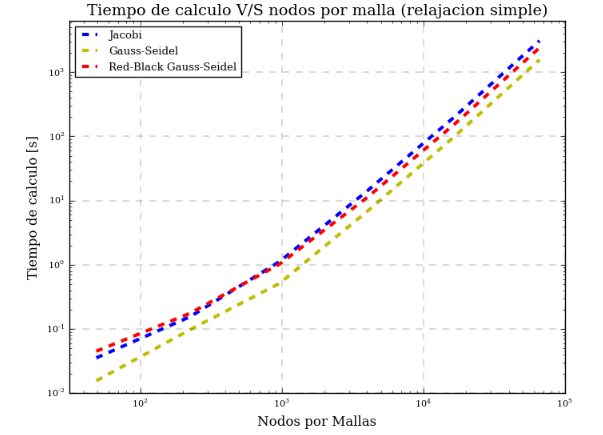
\includegraphics[scale=0.8]{img/tvsnsimple}
\caption{Complejidad algoritmica para métodos de relajación}
\label{comtvsnsimple}
\end{figure}

\begin{table}[H]
\centering
\caption{Tabla resumen para la aplicación de v-cycle con inyección}
\begin{tabular}[t]{|l|r|r|r|r|r|}
\hline
\multicolumn{ 1}{|c|}{Jacobi} & \multicolumn{1}{l|}{Nodos} & \multicolumn{1}{l|}{Tiempo [s]}& \multicolumn{1}{l|}{Ciclos} & \multicolumn{1}{c|}{$||r||_{\infty}$} & \multicolumn{1}{c|}{$||e||_{\infty}$} \\ \cline{ 2- 6}
\multicolumn{ 1}{|l|}{} &9 & 0.045602& 49 & 9.91E-09 & 0.0007639 \\ \cline{ 2- 6}
\multicolumn{ 1}{|l|}{} & 17 & 0.183961 & 184 &9.49E-09 & 0.0001967 \\ \cline{ 2- 6}
\multicolumn{ 1}{|l|}{} & 33 & 0.931226 & 667 &9.87E-09 & 4.92E-05 \\ \cline{ 2- 6}
\multicolumn{ 1}{|l|}{} & 65 & 5.984544 & 2383 &9.95E-09 & 1.23E-05 \\ \cline{ 2- 6}
\multicolumn{ 1}{|l|}{} & 129 & 49.432473 & 8382 &1.00E-08 & 3.07E-06 \\ \cline{ 2- 6}
\multicolumn{ 1}{|l|}{} & 257 & 568.544919 & 28924 & 1.00E-08 &7.69E-07 \\ \hline

\multicolumn{ 1}{|c|}{GS} & \multicolumn{1}{l|}{Nodos} & \multicolumn{1}{l|}{Tiempo [s]}& \multicolumn{1}{l|}{Ciclos} & \multicolumn{1}{c|}{$||r||_{\infty}$} & \multicolumn{1}{c|}{$||e||_{\infty}$} \\ \cline{ 2- 6}
\multicolumn{ 1}{|l|}{} &9 & 0.0091& 8 & 5.55E-09 & 0.0007639 \\ \cline{ 2- 6}
\multicolumn{ 1}{|l|}{} & 17 & 0.00928 & 8 &3.37E-09 & 0.0001967 \\ \cline{ 2- 6}
\multicolumn{ 1}{|l|}{} & 33 & 0.01050 & 8 &3.00E-09 & 4.92E-05 \\ \cline{ 2- 6}
\multicolumn{ 1}{|l|}{} & 65 & 0.02366& 8 & 2.84E-09 & 1,23E-05 \\ \cline{ 2- 6}
\multicolumn{ 1}{|l|}{} & 129 & 0.06263& 8 & 2.81E-08 & 3,07E-06 \\ \cline{ 2- 6}
\multicolumn{ 1}{|l|}{} & 257 & 0.15729& 8 & 2.81E-08 & 7.68E-07 \\ \hline

\multicolumn{ 1}{|c|}{RB GS} & \multicolumn{1}{l|}{Nodos} & \multicolumn{1}{l|}{Tiempo [s]}& \multicolumn{1}{l|}{Ciclos} & \multicolumn{1}{c|}{$||r||_{\infty}$} & \multicolumn{1}{c|}{$||e||_{\infty}$} \\ \cline{ 2- 6}
\multicolumn{ 1}{|l|}{} &9 & 0.012425& 9 & 6.59E-09 & 0.0007638829 \\ \cline{ 2- 6}
\multicolumn{ 1}{|l|}{} & 17 & 0.028025 & 17 &7.38E-09 & 0.0001967 \\ \cline{ 2- 6}
\multicolumn{ 1}{|l|}{} & 33 & 0.053658 & 23 &9.87E-09 & 4.92E-05 \\ \cline{ 2- 6}
\multicolumn{ 1}{|l|}{} & 65 & 0.253512 & 70 & 8.00E-09 & 1.23E-05 \\ \cline{ 2- 6}
\multicolumn{ 1}{|l|}{} & 129 & - & - & - & - \\ \cline{ 2- 6}
\multicolumn{ 1}{|l|}{} & 257 & - & - & - & - \\ \hline
\end{tabular}
\label{resumenvcin}
\end{table}

\begin{figure}
\centering
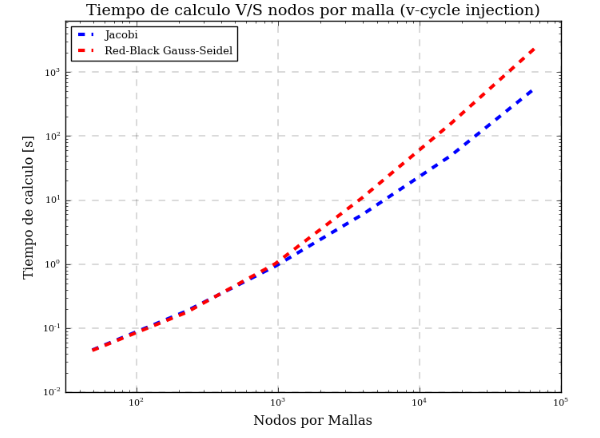
\includegraphics[scale=0.8]{img/tvsnvcin}
\caption{Complejidad algoritmica para v-cycle con inyección}
\label{comtvsnvcin}
\end{figure}

\begin{table}[H]
\centering
\caption{Tabla resumen para la aplicación de v-cycle con Full-Weighting}
\begin{tabular}[t]{|l|r|r|r|r|r|}
\hline
\multicolumn{ 1}{|c|}{Jacobi} & \multicolumn{1}{l|}{Nodos} & \multicolumn{1}{l|}{Tiempo [s]}& \multicolumn{1}{l|}{Ciclos} & \multicolumn{1}{c|}{$||r||_{\infty}$} & \multicolumn{1}{c|}{$||e||_{\infty}$} \\ \cline{ 2- 6}
\multicolumn{ 1}{|l|}{} &9 & 0.03758& 48 & 7.64E-09 & 0.0007639 \\ \cline{ 2- 6}
\multicolumn{ 1}{|l|}{} & 17 & 0.20320 & 175 & 9.82E-09 & 0.0001967 \\ \cline{ 2- 6}
\multicolumn{ 1}{|l|}{} & 33 & 0.93587 & 631 & 9.96E-09 & 4.92E-05 \\ \cline{ 2- 6}
\multicolumn{ 1}{|l|}{} & 65 & 5.72426 & 2239 & 9.98E-09 & 1.23E-05 \\ \cline{ 2- 6}
\multicolumn{ 1}{|l|}{} & 129 & 49.13004 & 7808 & 9.99E-08 & 3.07E-06 \\ \cline{ 2- 6}
\multicolumn{ 1}{|l|}{} & 257 & 537.07808 & 26945 & 1.00E-08 &7.68E-07 \\ \hline

\multicolumn{ 1}{|c|}{GS} & \multicolumn{1}{l|}{Nodos} & \multicolumn{1}{l|}{Tiempo [s]}& \multicolumn{1}{l|}{Ciclos} & \multicolumn{1}{c|}{$||r||_{\infty}$} & \multicolumn{1}{c|}{$||e||_{\infty}$} \\ \cline{ 2- 6}
\multicolumn{ 1}{|l|}{} &9 & 0.0110450 & 10 & 2.02E-09 & 0.0007639 \\ \cline{ 2- 6}
\multicolumn{ 1}{|l|}{} & 17 & 0.0134871 & 10 & 2.40E-09 & 0.0001967 \\ \cline{ 2- 6}
\multicolumn{ 1}{|l|}{} & 33 & 0.0178421 & 10 & 2.59E-09 & 4.92E-05 \\ \cline{ 2- 6}
\multicolumn{ 1}{|l|}{} & 65 & 0.0285549 & 10 & 2.64E-09 & 1,23E-05 \\ \cline{ 2- 6}
\multicolumn{ 1}{|l|}{} & 129 & 0.0721941 & 10 & 2.65E-08 & 3,07E-06 \\ \cline{ 2- 6}
\multicolumn{ 1}{|l|}{} & 257 & 0.213666 & 10 & 2.66E-08 & 7.68E-07 \\ \hline

\multicolumn{ 1}{|c|}{RB GS} & \multicolumn{1}{l|}{Nodos} & \multicolumn{1}{l|}{Tiempo [s]}& \multicolumn{1}{l|}{Ciclos} & \multicolumn{1}{c|}{$||r||_{\infty}$} & \multicolumn{1}{c|}{$||e||_{\infty}$} \\ \cline{ 2- 6}
\multicolumn{ 1}{|l|}{} &9 & 0.015742 & 10 & 7.87E-09 & 0.0007638829 \\ \cline{ 2- 6}
\multicolumn{ 1}{|l|}{} & 17 & 0.025217 & 11 & 2.53E-09 & 0.0001967 \\ \cline{ 2- 6}
\multicolumn{ 1}{|l|}{} & 33 & 0.035711 & 11 & 3.27E-09 & 4.92E-05 \\ \cline{ 2- 6}
\multicolumn{ 1}{|l|}{} & 65 & 0.051221 & 11 & 3.57E-09 & 1.23E-05 \\ \cline{ 2- 6}
\multicolumn{ 1}{|l|}{} & 129 & 0.101164 & 11 & 3.66E-09 & 3.07E-06 \\ \cline{ 2- 6}
\multicolumn{ 1}{|l|}{} & 257 & 0.288597 & 11 & 3.70E-09 & 7.68E-07 \\ \hline
\end{tabular}
\label{resumenvcfw}
\end{table}

\begin{figure}
\centering
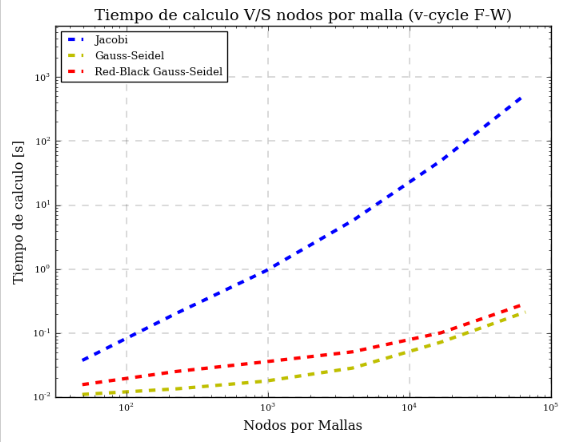
\includegraphics[scale=0.8]{img/tvsnvcfw}
\caption{Complejidad algoritmica para v-cycle con Full-Weighting}
\label{comtvsnvcfw}
\end{figure}

Para Multigrid, debido a que Gauss-Seilde tiene el mejor comportamiento, se recogen los resultados en base a esta forma de relajar.

\begin{table}[H]
\centering
\caption{Tabla resumen para la aplicación de Multigrid $\nu_0=5$, $\nu_1=10$, $\nu_2=10$}
\begin{tabular}[t]{|l|r|r|r|r|}
\hline
\multicolumn{5}{|c|}{Full-Weighting}\\ \hline
\multicolumn{ 1}{|c|}{GS} & \multicolumn{1}{l|}{Nodos} & \multicolumn{1}{l|}{Tiempo [s]} & \multicolumn{1}{c|}{$||r||_{\infty}$} & \multicolumn{1}{c|}{$||e||_{\infty}$} \\ \cline{ 2- 5}
\multicolumn{ 1}{|l|}{} &9 & 0.007142 & 2.53E-09 & 0.0007639 \\ \cline{ 2- 5}
\multicolumn{ 1}{|l|}{} & 17 & 0.011761 & 1.55E-09 & 0.0001967 \\ \cline{ 2- 5}
\multicolumn{ 1}{|l|}{} & 33 & 0.021827 & 3.08E-09 & 4.92E-05 \\ \cline{ 2- 5}
\multicolumn{ 1}{|l|}{} & 65 & 0.037276 & 3.66E-09 & 1,23E-05 \\ \cline{ 2- 5}
\multicolumn{ 1}{|l|}{} & 129 & 0.071036 & 3.84E-08 & 3,07E-06 \\ \cline{ 2- 5}
\multicolumn{ 1}{|l|}{} & 257 & 0.183730 & 3.92E-08 & 7.68E-07 \\ \hline
\multicolumn{5}{|c|}{Injection}\\ \hline
\multicolumn{ 1}{|c|}{GS} & \multicolumn{1}{l|}{Nodos} &\multicolumn{1}{l|}{Tiempo [s]}&  \multicolumn{1}{c|}{$||r||_{\infty}$} & \multicolumn{1}{c|}{$||e||_{\infty}$} \\ \cline{ 2- 5}
\multicolumn{1}{|l|}{} &9 & 0.0074651 & 7.17E-12 & 0.0007639 \\ \cline{ 2- 5}
\multicolumn{1}{|l|}{} & 17 & 0.0132601 & 2.55E-11 & 0.0001967 \\ \cline{ 2- 5}
\multicolumn{1}{|l|}{} & 33 & 0.0178909 & 3.25E-11 & 4.92E-05 \\ \cline{ 2- 5}
\multicolumn{ 1}{|l|}{} & 65 & 0.0314591 & 3.59E-11 & 1,23E-05 \\ \cline{ 2- 5}
\multicolumn{1}{|l|}{} & 129 & 0.0623319 & 3.72E-11 & 3,07E-06 \\ \cline{ 2- 5}
\multicolumn{1}{|l|}{} & 257 & 0.2000990 & 3.80E-11 & 7.68E-07 \\ \hline
\end{tabular}
\label{resumenmg10105}
\end{table}

\begin{table}[H]
\centering
\caption{Tabla resumen para la aplicación de Multigrid $\nu_0=4$, $\nu_1=10$, $\nu_2=10$}
\begin{tabular}[t]{|l|r|r|r|r|}
\hline
\multicolumn{5}{|c|}{Full-Weighting}\\ \hline
\multicolumn{ 1}{|c|}{GS} & \multicolumn{1}{l|}{Nodos} & \multicolumn{1}{l|}{Tiempo [s]} & \multicolumn{1}{c|}{$||r||_{\infty}$} & \multicolumn{1}{c|}{$||e||_{\infty}$} \\ \cline{ 2- 5}
\multicolumn{ 1}{|l|}{} &9 & 0.00757 & 2.54E-09 & 0.0007639 \\ \cline{ 2- 5}
\multicolumn{ 1}{|l|}{} & 17 & 0.01892 & 8.50E-08 & 0.0001967 \\ \cline{ 2- 5}
\multicolumn{ 1}{|l|}{} & 33 & 0.01766 & 1.56E-07 & 4.92E-05 \\ \cline{ 2- 5}
\multicolumn{ 1}{|l|}{} & 65 & 0.02522 & 1.89E-07 & 1,23E-05 \\ \cline{ 2- 5}
\multicolumn{ 1}{|l|}{} & 129 & 0.06966 & 2.05E-07 & 3,08E-06 \\ \cline{ 2- 5}
\multicolumn{ 1}{|l|}{} & 257 & 0.16068 & 2.09E-07 & 7.77E-07 \\ \hline
\multicolumn{5}{|c|}{Injection}\\ \hline
\multicolumn{ 1}{|c|}{GS} & \multicolumn{1}{l|}{Nodos} &\multicolumn{1}{l|}{Tiempo [s]}&  \multicolumn{1}{c|}{$||r||_{\infty}$} & \multicolumn{1}{c|}{$||e||_{\infty}$} \\ \cline{ 2- 5}
\multicolumn{1}{|l|}{} &9 & 0.004955 & 8.79E-10 & 0.0007639 \\ \cline{ 2- 5}
\multicolumn{1}{|l|}{} & 17 & 0.011606 & 3.06E-09 & 0.0001967 \\ \cline{ 2- 5}
\multicolumn{1}{|l|}{} & 33 & 0.018774 & 3.57E-09 & 4.92E-05 \\ \cline{ 2- 5}
\multicolumn{ 1}{|l|}{} & 65 & 0.034140 & 3.86E-09 & 1,23E-05 \\ \cline{ 2- 5}
\multicolumn{1}{|l|}{} & 129 & 0.062984 & 3.97E-09 & 3,07E-06 \\ \cline{ 2- 5}
\multicolumn{1}{|l|}{} & 257 & 0.152861 & 4.00E-09 & 7.68E-07 \\ \hline
\end{tabular}
\label{resumenmg10104}
\end{table}





\begin{table}[H]
\centering
\caption{Comparación de la complejidad algorimica de los tres casos con $Gauss-Seidel$. Multigrid con $\nu_0=5$,$\nu_1=10$,$\nu_2=10$  }
\begin{tabular}[t]{|c|c|}
\hline
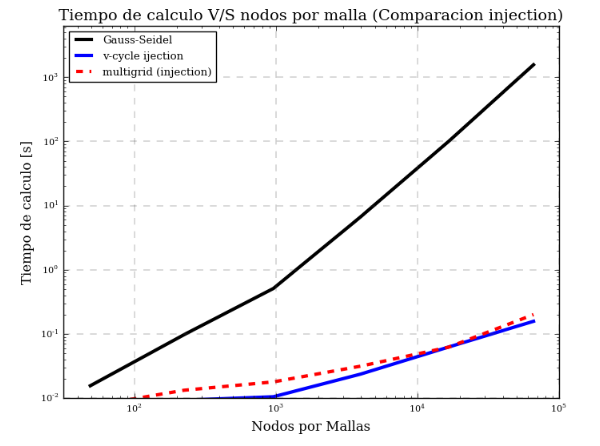
\includegraphics[scale=0.55]{img/tvsncompin}
&
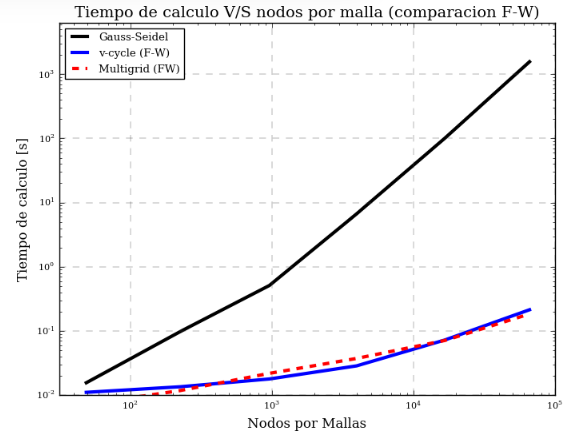
\includegraphics[scale=0.55]{img/tvsncompfw}\\
\hline
\end{tabular}
\label{comp10105}

\end{table}

\begin{table}[H]
\centering
\caption{Comparación de la complejidad algorimica de los tres casos con $Gauss-Seidel$. Multigrid con $\nu_0=4$,$\nu_1=10$,$\nu_2=10$  }
\begin{tabular}[t]{|c|c|}
\hline
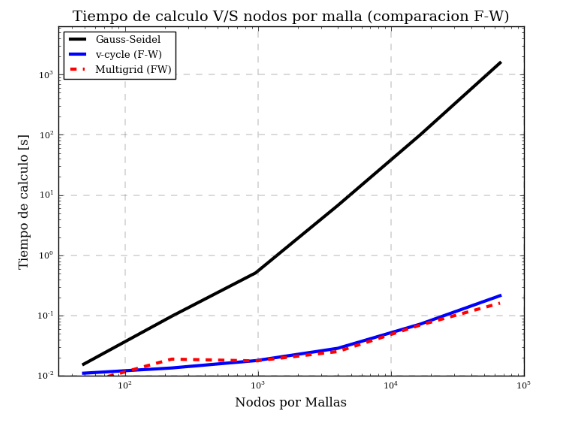
\includegraphics[scale=0.58]{img/tvsncompin10104}
&
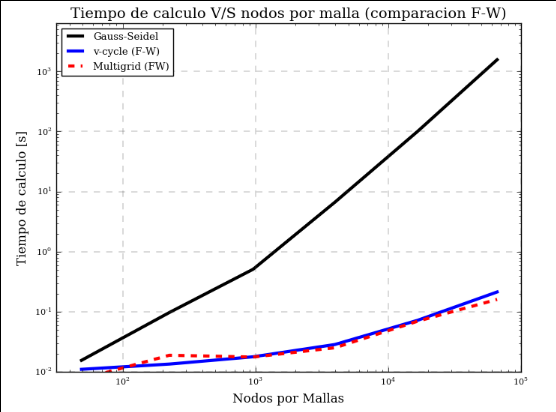
\includegraphics[scale=0.58]{img/tvsncompfw10104}\\
\hline
\end{tabular}
\label{comp10104}

\end{table}

\subsubsection{Comparación multi malla a iguales condiciones}

\begin{table}[H]
\centering
\caption{Reportes para comparar v-cycle con multigrid usando inyección para $\nu_0=4$, $\nu_1=10$, $\nu_2=10$}
\begin{tabular}[t]{|c|c|c|}
\hline
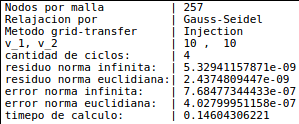
\includegraphics[scale=0.65]{img/reportefmg/reportevc257}
&
\includegraphics[scale=0.65]{img/reportefmg/reportevc513}
&
\includegraphics[scale=0.65]{img/reportefmg/reportevc1025}\\
\hline
\includegraphics[scale=0.65]{img/reportefmg/reportemg257}
&
\includegraphics[scale=0.65]{img/reportefmg/reportemg513}
&
\includegraphics[scale=0.65]{img/reportefmg/reportemg1025}\\
\hline

\end{tabular}

\label{reportesvcvsmg}
\end{table}

\newpage

\section{Análisis y Conclusiones}

En primer lugar, comparando los gráficos de la Figura \ref{cualitteorico} con las figuras del Cuadro \ref{cualitrelaxsimple}, se observa que al menos de forma cualitativa los códigos implementados para resolver $Jacobi$, $Gauss-Seidel$ y $Red-Black Gauss-Seidel$ son capaces de dar una buena aproximación $v$ del campo escalar $u$. De el mismo modo, para $V-cycle$, usando $Full-Weighting$ cualitativamente las relajaciones también son capaces de representar el comportamiento de $u$ mediante aproximaciones de $v$ para los valres de $\nu_0$, $\nu_1$ y $\nu_2$ que se indican en el Cuadro \ref{cualitvc}, sin embargo, en dicho cuadro se puede observar que el caso en que se prueba el inyección para $129$ nodos por eje, el código no es capaz de calcular los valores de $v$ que aproximan $u$ para $Red-Black$ $Gauss-Seidel$.\\
\indent Antes de pasar al análisis cualitativo de multigrid, se pretende contrastar lo visto anteriormente con la cuantificación de los análisis llevados a cabo anteriormente. Se observa en los cuadros \ref{resumenrelaximple}, \ref{resumenvcin}, \ref{resumenvcfw} que los errores con respecto al resultado real se reducen cuando el residuo alcanza la tolerancia, esto explica y concuerda con los mapas de contorno que se observan en las figuras expuestas en lo cuados \ref{cualitrelaxsimple} y \ref{cualitvc} y de igual modo, para nodos mayores a $129$ por eje, el calculo de $Red-Black$ $Gauss-Seidel$ no se puede llevar a cabo, o mejor dicho diverge. En la tabla de la Figura \ref{tablaejemplolibro} extraída del libro \cite{converfact} Se observa que para los distintos métodos de relajación, dependiendo de la combinación de $\nu_1$ y $\nu_2$ los resultados de la relajación pueden diverger. Aquí se observa que jacobi, con $\nu_1=1$ y $\nu_2=0$, diverge, pero a medida que se incrementan estos valores, este recupera la convergencia para el caso en que se use inyección.\\

\begin{figure}[H]
\centering
\includegraphics[scale=0.6]{img/tablalibro}
\caption{Tabla de comparación de factores de comnvergencia extraido del libro $A$ $Multigrif$ $Tutorial$ \cite{converfact}}
\label{tablaejemplolibro}
\end{figure}

\indent Lo mencionado anteriormente da pistas de que el metodo de $Red-Black$ $Gauss-Seidel$ puede llegar a converger, sin embargo, se probaron combinaciones de $\nu_1$ y $\nu_2$ hasta llegar a $\nu_1=10$ y $\nu_2=10$, y aun así este no converge. Esto puede significar que el factor de convergencia para forma de relajar sigue siendo malo, pero no se quiso probar para un mayor numero de relajaciones ya que se hacia cada vez mas lento por lo cual carece de sentido usar dicha combinación de métodos.

\begin{figure}[H]
\centering
\includegraphics[scale=1]{img/reportefmg/reportevcrbgsin129}
\caption{Resporte donde se ve que el ciclo-v usando $Red-Black$ $Gauss-Seidel$ aun diverge con $\nu_1=10$ y $\nu_2=10$}
\label{reporterbgs129in}
\end{figure}

\indent En cuanto a la complejidad algoritmica, los gráficos de las Figuras \ref{comtvsnsimple}, \ref{comtvsnvcin} y \ref{comtvsnvcfw} muestra que el orden tiempo que se demoran los calculos es de $o{n^2}$ y $o{n\cdot log(n)}$. Si se hace el ejercicio de predecir el tiempo para los datos del cuadro \ref{resumenrelaximple} es posible ver que el si la cantidad de nodos aumenta cuatro veces, el tiempo de la siguiente iteración aumenta dieciséis veces, lo cual, si bien no entrega el tiempo exacto, la predicción es una buena aproximación del tiempo que se demorara. En cuanto al resultado de los cuadros \ref{resumenvcin} y \ref{comtvsnvcfw}, la predicción de los tiempos para $Jacobi$ no se cumplen, pero para $Gauss-Seidel$ si y en el caso de $Red-Black$ $Gauss-Seidel$ solo se cumple si se ocupa $Full-Weighting$. De todos modos el gráfico de la Figura \ref{comtvsnvcin} demuestra que hay un comportamiento de tipo algoritmico para la complejidad de Jacobi, el que no se puda predecir a partir de $n\cdot log(n) $ es debido a que se aprecia claramente, ya sea en los cuadros \ref{resumenvcin} y \ref{resumenvcfw} que el tiempo que demora depende de la cantidad ciclos para este método de relajación, lo cual en el caso de $Gauss-Seidel$ y $Red-Black$ $Gauss-Seidel$ hay indicios de que el residuo cumple con la tolerancia para una cantidad fija de ciclos, o con una variación muy leve en cuanto a la cantidad de ciclos.\\
\indent Por todo lo expuesto anteriormente, se observa que el método de relajación que mejor se comporta utilizando métodos de multimalla como $V-cycle$ es $Gauss-Seidel$. En base a esta conclusión el análisis para $Full-Multigrid$ se hace únicamente con este tipo de relajación (y con la finalidad de no extender en demasía el informe).\\
\indent Si se observan las figuras del Cuadro \ref{cualitmg221}, el comportamiento cualitativo de $v$ no se acerca al teóricamente esperado por lo cual, se concluye que las condiciones de $\nu_0=1$, $\nu_1=2$ y $\nu_2=2$ no son suficientes, esto se debe a que $Multigrid$ en si no realiza mas de un ciclo y dentro de ese ciclo debe hacer la cantidad de relajaciones suficiente para que $v$ se aproxime al valor teórico. Debido a que claramente esta combinación no fue suficiente, es necesario modificar los valores $nu$ para obtener mejores resultados.


\newpage

\begin{thebibliography}{9}
\bibitem{iter}\textsc{William L. Briggs, Van Emden Henson, Steve F. McCormick} \textit{Chapter 2: Basic Iterative Methos}, \textit{A Multigrid Tutorial} \textsc{Second Edition}\textsc{Editorial: SIAM} 15 de Noviembre de 1999, Boulder Colorado, \textsc{(Page: 7 - 30)}

\bibitem{converfact}\textsc{William L. Briggs, Van Emden Henson, Steve F. McCormick} \textit{Chapter 4: implementation}, \textit{A Multigrid Tutorial} \textsc{Second Edition}\textsc{Editorial: SIAM} 15 de Noviembre de 1999, Boulder Colorado, \textsc{(Page: 58 - 85)}

\end{thebibliography}


\end{document}



